\section{The pan-assembly graph}

The following graph definitions respect the sequence graph definition:

\begin{definition}
  {Sequence graph}{sequence_graph} Let
  \(G = (V_{t}\cup V_{h}, E_{\mathcal{S}} \cup \ELinks{})\) be a multi-undirected
  graph (multigraph) where:

  \begin{itemize}
    \item \(\mathcal{S}\) is the set of sequences

    \item \(\Links{}\) is the multiset of links between oriented sequences

    \item vertices from \(V_{t}\) and \(V_{h}\) represent respectively the tails
      and heads of the sequences

    \item sequence-edges from \(E_{\mathcal{S}}\) represent the sequences and connect
      two extremities of the same sequence (\(E_{\mathcal{S}}\) is a perfect
      matching of the vertices)

    \item link-edges from the multi-link-edge set \(\ELinks{}\) represent
      the links between the sequences
  \end{itemize}
\end{definition}

Let \(Asm_{1}\) and \(Asm_{2}\) be two assembly methods, their respective contig set \(\Contigs{}_{1}\) and \(\Contigs{}_{2}\) and their respective link set \(\Links{}_{1}\) and \(\Links{}_{2}\).
\(G_{1}= (V_{1t}\cup V_{1h}, E_{\Contigs{}_1}\cup E_{\Links{}_1})\) and \(G_{2}= (V_{2t}\cup V_{2h}, E_{\Contigs{}_2}\cup E_{\Links{}_2})\) respectively denote the assembly graphs of \(Asm_{1}\) and \(Asm_{2}\). By \(\Contigs{} = \Contigs{}_1 \cup \Contigs{}_2\) we denote the set of all the contigs.

We denote by the sequence graph \(PG = (V = V_t \cup V_h, E = \EFrags{} \cup \ELinks{})\) the pan-assembly graph, where \(\Fragments{}\) is the set of pangenome fragments.

\subsection{Contigs in the pan-assembly graph}

Given a contig \(c\) in the set of contigs \(\Contigs{} = \Contigs{}_1 \cup \Contigs{}_2\) from the two assemblers (by \(c^-\) we denote the reverse).
In the pan-assembly graph \(PG\), there exists a unique sequence \(p_c\) of vertices in \(V\) corresponding to the contig \(c\).

\begin{notebox}
  Each sequence \(p_c\) can be decomposed as a fragment-edge --- link-edge alternate, beginning from and ending to a fragment-edge.
\end{notebox}

We denote by \(A(p_c)\) or \(A(c)\) the set of directed link-edges (link-arcs) composing contig \(c\).

\begin{notebox}
  By \(A(c^-)\) we denote the set of link-arcs composing the reverse of \(c\).
\end{notebox}

For a contig \(c \in \Contigs{}\), \(\Fragments{}(c) \subset \Fragments{}\) is the set of all fragments of \(c\).

\subsubsection{Contig properties}

Each contig is associated with three properties: its coverage, its plasmidness and a set of GC penalties depending on GC content intervals.

In the following, \(c \in \Contigs{}\) is a contig.

\begin{definition}{Contig coverage}{contig_coverage}
  By \(\cov{c} \in \Reals_{>0}\) we denote the coverage of \(c\).
  It corresponds to the average base coverage of the contig normalized by the median coverage of the contigs in the whole assembly.
\end{definition}

\begin{definition}{Contig GC probability score}{contig_GC_score}
  \begin{newfeatbox}
    We do not normalize the probabilities by the sum of the \(P(b|n,l)\) over all \(b \in K\) as in~\cite{manePlasBinflowFlowbasedMILP2023}. We normalize them according to the maximum among them.
  \end{newfeatbox}
  Let \(c \in \Contigs{}\) be a contig and \(b\) be a GC content interval.
  By \(\gcscore{c}{b} \in [-1, 1]\) we denote the GC probability score of the contig \(c\) according to the GC content interval \(b\):
  \[
    \gcscore{c}{b} = 2 \frac{\Pr(n|b,l)\Pr(b)}{\max\limits_{b' \in K}\Set*{\Pr(n|b',l)\Pr(b')}} - 1
  \]
  Where \(K\) is the set of GC content intervals, \(n\) is the number of GC in the contig of length \(l\), and \(\Pr(n|b,l)\) is calculated as described in~\cite{manePlasBinflowFlowbasedMILP2023}, Section 2.5.1.

  \begin{fixmebox}
    Adapt the correction constraints according to the new score definition.
  \end{fixmebox}
\end{definition}

\begin{definition}{Contig plasmidness}{contig_plasmidness}
  Let \(c \in \Contigs{}\) be a contig.
  By \(\plm{c} \in [0, 1]\) we denote its plasmidness score.
  A plasmid sequence classifier can provid these scores.
\end{definition}

\subsection{The set of fragments}

A pangenome fragment can come from:

\begin{enumerate}
  \item a unique contig of \(Asm_1\)

  \item a unique contig of \(Asm_2\)

  \item at least one contig of \(Asm_1\) and at least one contig of \(Asm_2\)
\end{enumerate}

\begin{missingproofbox}
  There is no share such that all its contigs come from the same assembler
\end{missingproofbox}

In cases 1 and 2, the fragment is defined as a \emph{subcontig}, while in case 3 it is defined as a shared subcontig (\emph{a share}).

For a fragment \(i \in \Fragments{}\), \(\Contigs{}(i) \subset \Contigs{}\) denotes the set of contigs from which \(i\) comes from. The fragment \(i\) is a subcontig if and only if \(|\Contigs{}(i)| = 1\), otherwise \(i\) is a share if and only if \(|\Contigs{}(i)| > 1\).
The extremity vertices in \(V\) of a fragment \(i \in \Fragments{}\) are provided by \(i_t \in V_t\) and \(i_h \in V_h\) (note that \(\Set{i_t, i_h} \in \EFrags{}\)). Reversely, \(vfrag \colon V \tosur \Fragments{}\) gives the fragment associated to one of its extremity vertices.

\subsubsection{Fragment properties}

Each fragment is associated with three properties: its coverage, its plasmidness and a set of GC penalties depending on GC content intervals.

\begin{definition}{Fragment coverage}{fragment_coverage}
  \begin{todobox}
    Explain why we do not normalize as Cédric Chauve proposed.
  \end{todobox}
  Let \(i \in \Fragments{}\) be a fragment.
  By \(\cov{i} \in \Reals{}_{>0}\) we denote its coverage:
  \[
    \cov{i} = \max_{c \in \Contigs{}(i)}\Set*{\cov{c}}
  \]
\end{definition}

\begin{newfeatbox}
  While PlasBin-flow uses a GC content penalty, we use a GC score

  \begin{questionbox}
    Before we had a penalty.
    The flow can pass through loops and cycles, without changing the total flow (because of the conservation constraints). But the GC content penalties prevent us to use more fragments otherwise the objective value is most likely to decrease.

    That can explain why some bins are split into several bins.
  \end{questionbox}

  \begin{questionbox}
    In the one hand, computing the fragment GC penalties from the contigs, and correct the penalties for the share, favours to keep the original contigs.

    Computing the fragment GC penalties from the contigs means we trust the contig assemblies (as in the formula, the length parameter is the length of the contig, not these of its fragments)

    In the other hand, recomputing the fragment GC penalties and thus using as the length parameter the length of the fragment may result in a strong statistical bias for short fragments.

    \begin{notebox}
      Here we chose to recompute the GC probabilities without taking into account from which contigs a fragment belongs.
    \end{notebox}
  \end{questionbox}
\end{newfeatbox}

\begin{definition}{Fragment GC score}{fragment_GC_score}
  Let \(i \in \Fragments{}\) be a fragment and \(b\) be a GC content interval.
  By \(\gcscore{i}{b} \in [-1, 1]\) we denote the GC score of the fragment \(i\) according to the GC content interval \(b\):
  \[
    \gcscore{i}{b} = 2 \frac{\Pr(n|b,l)\Pr(b)}{\max\limits_{b' \in K}\Set*{\Pr(n|b',l)\Pr(b')}} - 1
  \]
  Where \(K\) is the set of GC content intervals, \(n\) is the number of GC in the fragment of length \(l\), and \(\Pr(n|b,l)\) is calculated as described in~\cite{manePlasBinflowFlowbasedMILP2023}, Section 2.5.1.

  \begin{fixmebox}
    Adapt the correction constraints according to the new score definition.
  \end{fixmebox}
\end{definition}

\begin{definition}{Fragment plasmidness}{fragment_plasmidness}
  Let \(i \in \Fragments{}\) be a fragment.
  By \(\plm{i} \in [-1, 1]\) we denote its plasmidness score, such that:
  \[
    \plm{i} = \frac{ 1 }{ |\Contigs{}(i)| } \sum_{c \in \Contigs{}(i)} \frac{ |i| }{ |c| }\plm{c}
  \]
\end{definition}

\begin{definition}{Seed fragments}{seed_fragments}
  The set \(\SeedFrags{} \subset \Fragments{}\) contains the seed fragments.
  Seed fragments are fragments likely to define one or several bins.
  A bin can contain several seed fragments.
\end{definition}

\subsection{The pan-assembly links}

A link in the multi-link-edge set \(\ELinks{}\) is either of two types:
\begin{description}[style=nextline]
  \item[Pangenome link] A link connecting two fragments from the same contig, thus that can connect:
    \begin{itemize}
      \item two fragments from two contigs of different assemblers
      \item two fragments from two contigs of the same assembler
    \end{itemize}
  \item[Assembly link] A link connecting two fragments from two contigs of the same assembler which were linked in the original assembly graph
\end{description}

\Cref{fig:panasm_multi-edges} illustrates some multi-edge cases.

\begin{figure}[htb]
  \centering
  \begin{subfigure}[b]{0.45\linewidth}
    \centering
    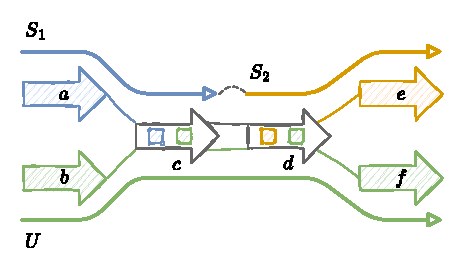
\includegraphics[width=\linewidth]{pan-assembly_graph/img/panassembly_graph-multi-edges_asm-pan.pdf}
    \caption{Assembly-Pangenome}\label{subfig:panasm_asm-pan}
  \end{subfigure}
  \hfill
  \begin{subfigure}[b]{0.45\linewidth}
    \centering
    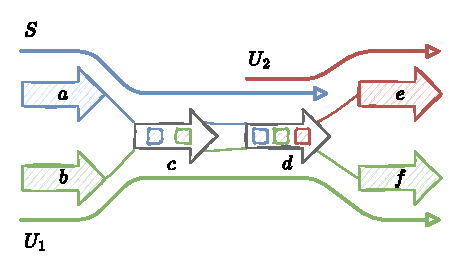
\includegraphics[width=\linewidth]{pan-assembly_graph/img/panassembly_graph-multi-edges_pan-pan.pdf}
    \caption{Pangenome-Pangenome}\label{subfig:panasm_pan-pan}
  \end{subfigure}
  \figurecaption{Multi-edge examples in the pan-assembly graph.}{%
    Arrows represent (oriented) sequences.
    Heavy ones represent fragments and thin ones represent the contigs.
    \Subref{subfig:panasm_asm-pan}
    Contig \(U\) comes from Unicycler while contigs \(S_1\) and \(S_2\) come from SKESA.
    Fragment set of \(U\) is \( \Fragments(U) = \{b, c, d, f\} \), and these of \(S_1\) and \(S_2\) are respectively \( \Fragments(S_1) = \{a, c\} \) and \( \Fragments(S_2) = \{d, e\} \).
    For example, green link \((c, d) \in \Links{}\) is a pangenome link while grey link \((c, d) \in \Links{}\) is an assembly link.
    \Subref{subfig:panasm_pan-pan}
    Contig \(S\) comes from SKESA, defined by \( \Fragments(S) = \{a, c, d\} \), while contigs \(U_1\) and \(U_2\) come from Unicycler, respectively defined by \( \Fragments(U_1) = \{b, c, d\} \) and \( \Fragments(U_2) = \{d, e\} \).
    Both blue and green multi-links \((c, d)\) are pangenome links, and they respectively connect fragments of contigs \(S\) and \(U_1\).
    However, they enable to connect a subpart of \(U_1\) to contig \(U_2\).
  }\label{fig:panasm_multi-edges}
\end{figure}

\subsection{Converting the multigraph to a simple graph}

We can convert the original pan-assembly graph, which is a multigraph, to a simple graph by merging all the multi-edges in one.

It consists in a priori merging all the multi-links between the fragments.
When the multi-links are of different types, we choose to type the link resulting from the merge as an assembly link.

\begin{notebox}
  Now, for each contig \(c \in \mathcal{C}\), the sets \(A_\Links{}(c)\) and \(A_\Links{}(c^-)\) do not contain the multi-edges but only the edges resulting from the merge of them, so that \(|A_\Links{}(c)| = |A_\Links{}(c^-)| = |\Fragments{}(c)| - 1\).
\end{notebox}

In the following, we consider \(PG\) to be the simple graph resulting from the merge of the multi-edges in \ELinks{}.
